\documentclass{standalone}
\usepackage[dvipsnames]{xcolor}
\usepackage{tikz}
\usepackage{fix-cm}
\setlength{\parskip}{0pt}
\setlength{\baselineskip}{0pt}
%\usetikzlibrary{fit}
\usetikzlibrary{calc}
\usetikzlibrary{decorations.markings}
\usetikzlibrary{decorations.shapes}
\usetikzlibrary{decorations.pathreplacing}
\usetikzlibrary{intersections}
\tikzset{%
  from end of path/.style={
    insert path={
      \pgfextra{%
        \expandafter\pgfprocesspathextractpoints%
          \csname tikz@intersect@path@name@#1\endcsname%
        \pgfpointlastonpath%
        \pgfgetlastxy\lastx\lasty
      }
      (\lastx,\lasty)
}}}
\tikzset{-dot-/.style={decoration={
  markings,
  mark=at position #1 with {\fill[color=red] circle (0.5mm);}},postaction={decorate}}} %%% in this line added a ;

\begin{document}
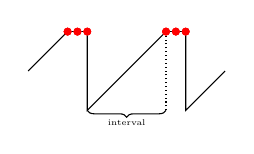
\begin{tikzpicture}
\draw[name path=A] (0,0.5)-- ++(0.5, 0.5);
\draw[from end of path=A, name path=B, -dot-=0, -dot-=0.5, -dot-=1] -- ++(0.25,0);
\draw[from end of path=B, name path=C] ++(0,-0.5mm) -- ++(0,-0.95cm) -- ++(1,1);
\draw[from end of path=C, name path=D, -dot-=0, -dot-=0.5, -dot-=1] -- ++(0.25,0);
\draw[from end of path=D, name path=D] ++(0,-0.5mm) -- ++(0,-0.95cm) -- ++(0.5,0.5);
\draw[draw,decorate,decoration={brace,mirror}] (0.75,0) -- (1.75,0) node [inner sep=0, outer sep=0,midway,below,yshift=-1.25mm] {\fontsize{3pt}{0}\selectfont interval};
\draw[densely dotted] (1.75,0) -- (1.75,0.95);
\end{tikzpicture}
\end{document}